\section{Numerical microlensing magnification maps}\label{sec:numerics}

Having used the simple model of an ideal fold to gain insight, we now
move to the numerical computation of microlensing light curves with
realistic mass distributions.  For this we we used the microlensing
code by \cite{1999A&A...346L...5W}.

The code uses a ray-shooting technique to compute the gravitational
lensing effect of a mass distribution consisting of (a)~a smooth
component and (b)~a random distribution of point masses representing
stars.  The ray shooting maps a grid of $\vec\theta$ to $\vec\beta$
using the lens equation (\ref{eqn:lens}).  That is, the rays are shot
from the observer back to the source.

For the computation of the individual deflection angles
$\vec\alpha(\vec\theta)$ a heirarchical or tree method is used.  The
positions of all lensing masses are put into a grid of $\vec\theta$.
Each grid cell is subdivided into four smaller squares recursively
until every cell contains only one mass.  Nearby masses are added
individually, while distance masses are clumped into larger grid cells
whose net contribution is approximated by its first few multipole
moments.  Scaled units are used, with the constant pre-factor in the
deflection angle (\ref{eqn:alpha}) separated out.

The result of ray shooting is a pixel map on the $\vec\beta$ plane of
the number of lightrays which arrive at the source plane from a
particular observer.  This intermediate result is effectively a
magnification map on the source plane.  Once the map is created, the
lightcurve can be obtained by specifying the transit path of the
source across the map.  At each point on this transit line, the code
computes equation (\ref{eqn:ft2d}) convolving the brightness
distribution of the source with the magnification pattern of the map.
In real life, not only are both lens and source moving, but the lens
lens configuration, and with it the magnification pattern, is also
changing with time.  While the first subtlety is taken care of by a
coordinate transformation in this analysis, for the second one the
lens configuration is assumed to be constant in time.

When generating the magnification map depicted in
Figure~\ref{fig:magnification_map}, which is used in our analysis
below, only two point masses were included.  This was done in order to
have clean fold caustics.  For the computation of the actual
lightcurve, the code was modified to also allow for crescent shaped
images specified through the parameter set $R_p,R_n,a,b$. Here $R_p$
denotes the outer radius of the crescent and $R_n$ the inner one. The
orientation of the source image with respect to the magnification map
is specified by the parameters $a$ and $b$ as the shift of the center
of the inner disk from the center of the outer disk in $x$- and
$y$-direction respectively. In the original version of the code,
gaussian and disk shaped images where already implemented. Those are
completely characterised by the single parameter $R_p$. The values of
the parameters are specified in pixel units corresponding to the
magnification map. Further one needs to specify the start and end
point coordinates of the path, which the center of the source image
follows through the magnification map (see the depiction in figure
\ref{fig:magnification_map}). Hence the points along this path are
specified through the number of timesteps for which the computation of
the brightness is to be carried out. Those points correspond to the
actual measurement of the brightness of an object in the observational
case. For each timestep the two-dimensional convolution of equation
\ref{eqn:ft2d} is carried out numerically for the position of the
source on the magnification map.

For the purpose of this analysis it was desirable to mimic the
analytical behaviour of a simple fold as much as possible, for
comparing the numerical result with the analytical one, therefore the
path of the source was chosen, so that it intersects the border of the
caustic perpendicularly, and on a point where the border is a fold
caustic.

\subsection{Microlensing a simulated image of M87}

\begin{figure}
\centering
        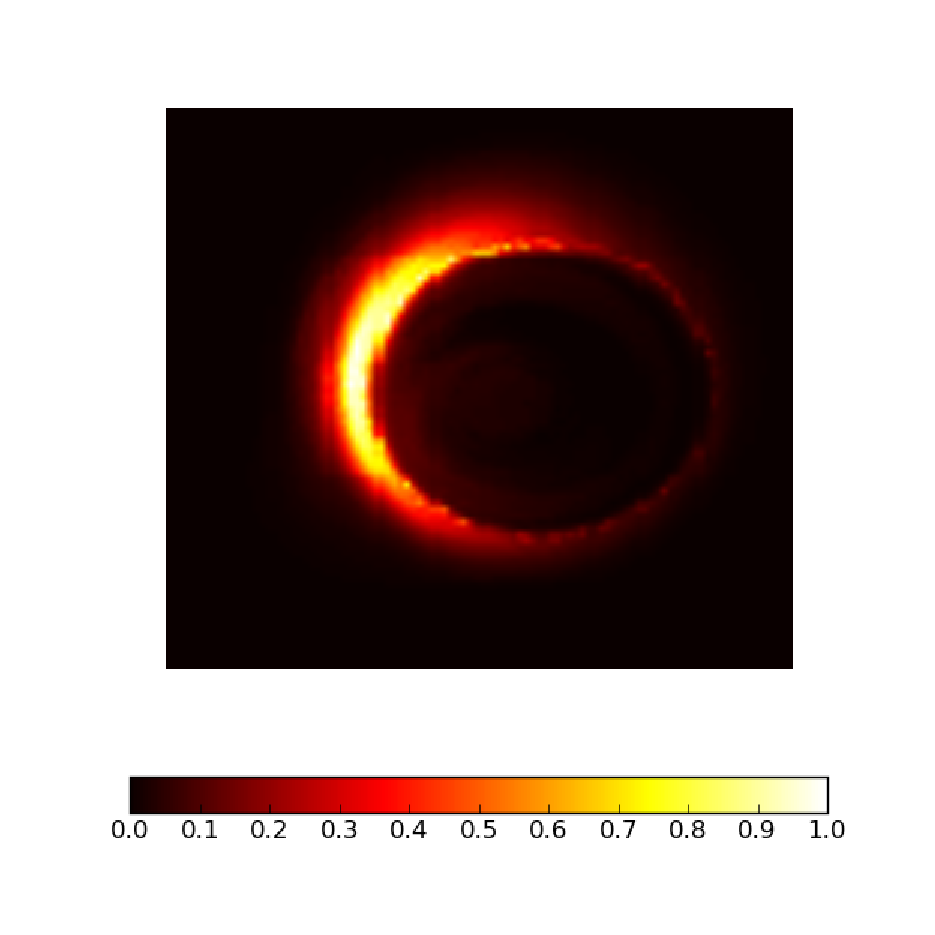
\includegraphics[width = 0.48\textwidth]{figures/M87_image.eps}
\caption{\label{fig:M87_image} The simulated image of M87's black hole
  sillouette obtained by \citep{2012MNRAS.421.1517D} from a GRMHD
  simulation presented in \citep{2009MNRAS.394L.126M}. The color bar
  is linear and scaled to reach value 1 for the maximum
  brightness. Points p2 and p3, mark the start and end of the
  equivalent dark disk and are associated to the moment of their
  overlap with the caustic t2 and t3.}
\end{figure}

\cite{2012MNRAS.421.1517D} have created a radiative image of M87 based on the GRMHD simulations presented in \citep{2009MNRAS.394L.126M}. The respective image, reproduced in figure \ref{fig:M87_image}, has been projected to a 1D profile associated to the perpendicular direction to a fold caustic approaching the image from the right. The projection is presented in the left panel of figure 10. The amplification values of the flux of light corresponding to a microlensing event are presented in the right panel of figure 10. In general the behaviour of the lightcurve is similar to the geometric crescent source with the caveat that the outer regions surrounding the luminous parts of the image have non-zero flux and thus are more extended than the simplified source model.

\begin{figure}
\centering
	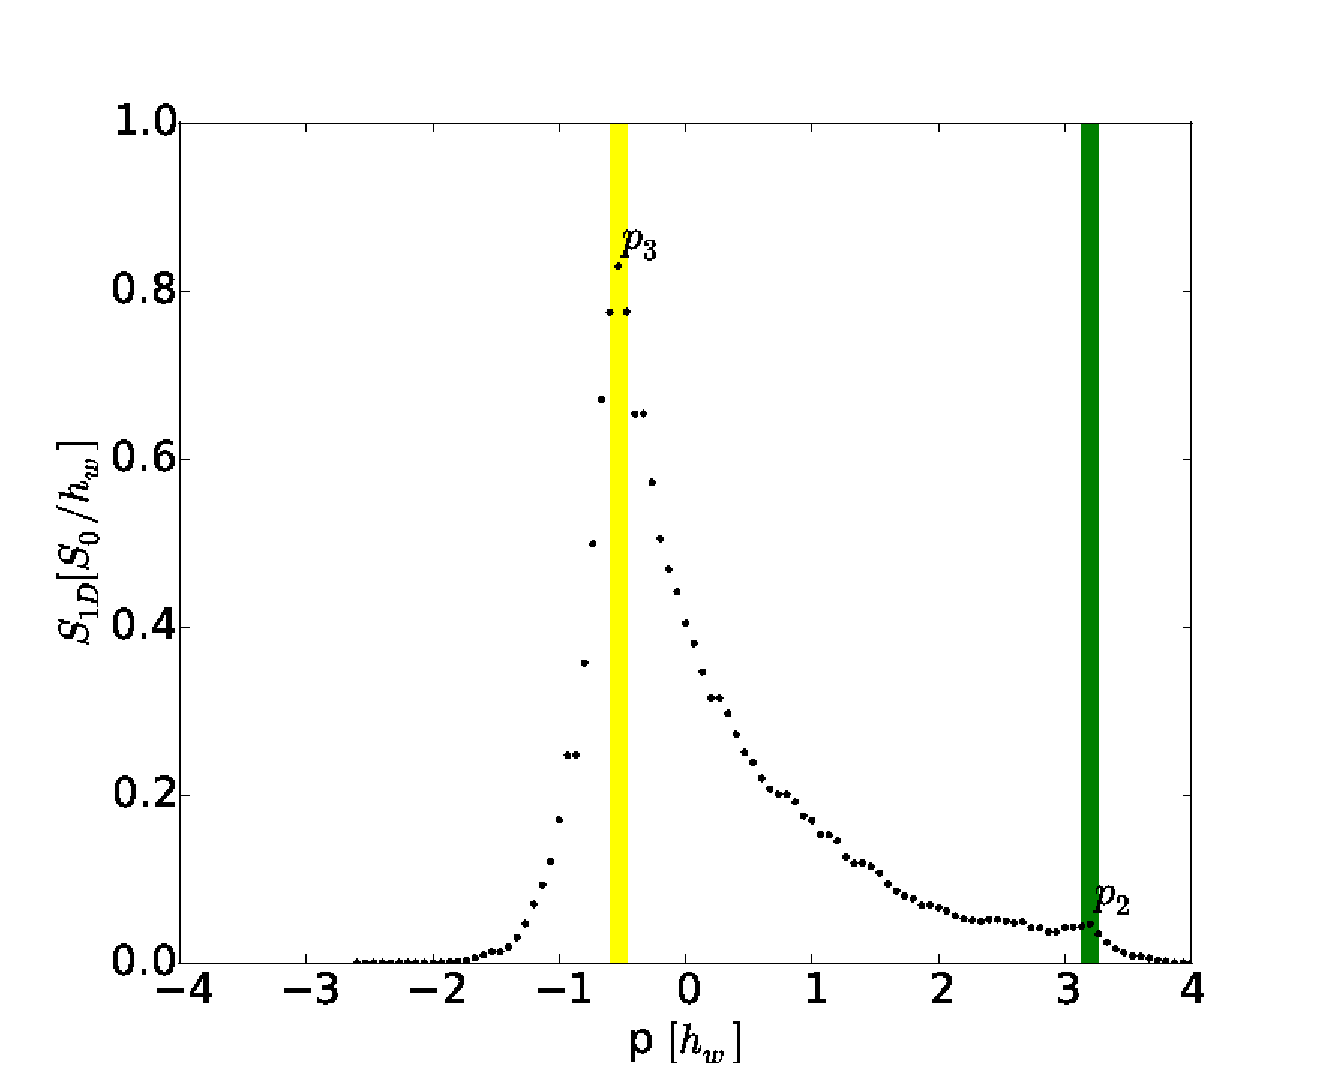
\includegraphics[width = 0.48\textwidth]{figures/M87_shape.eps}
        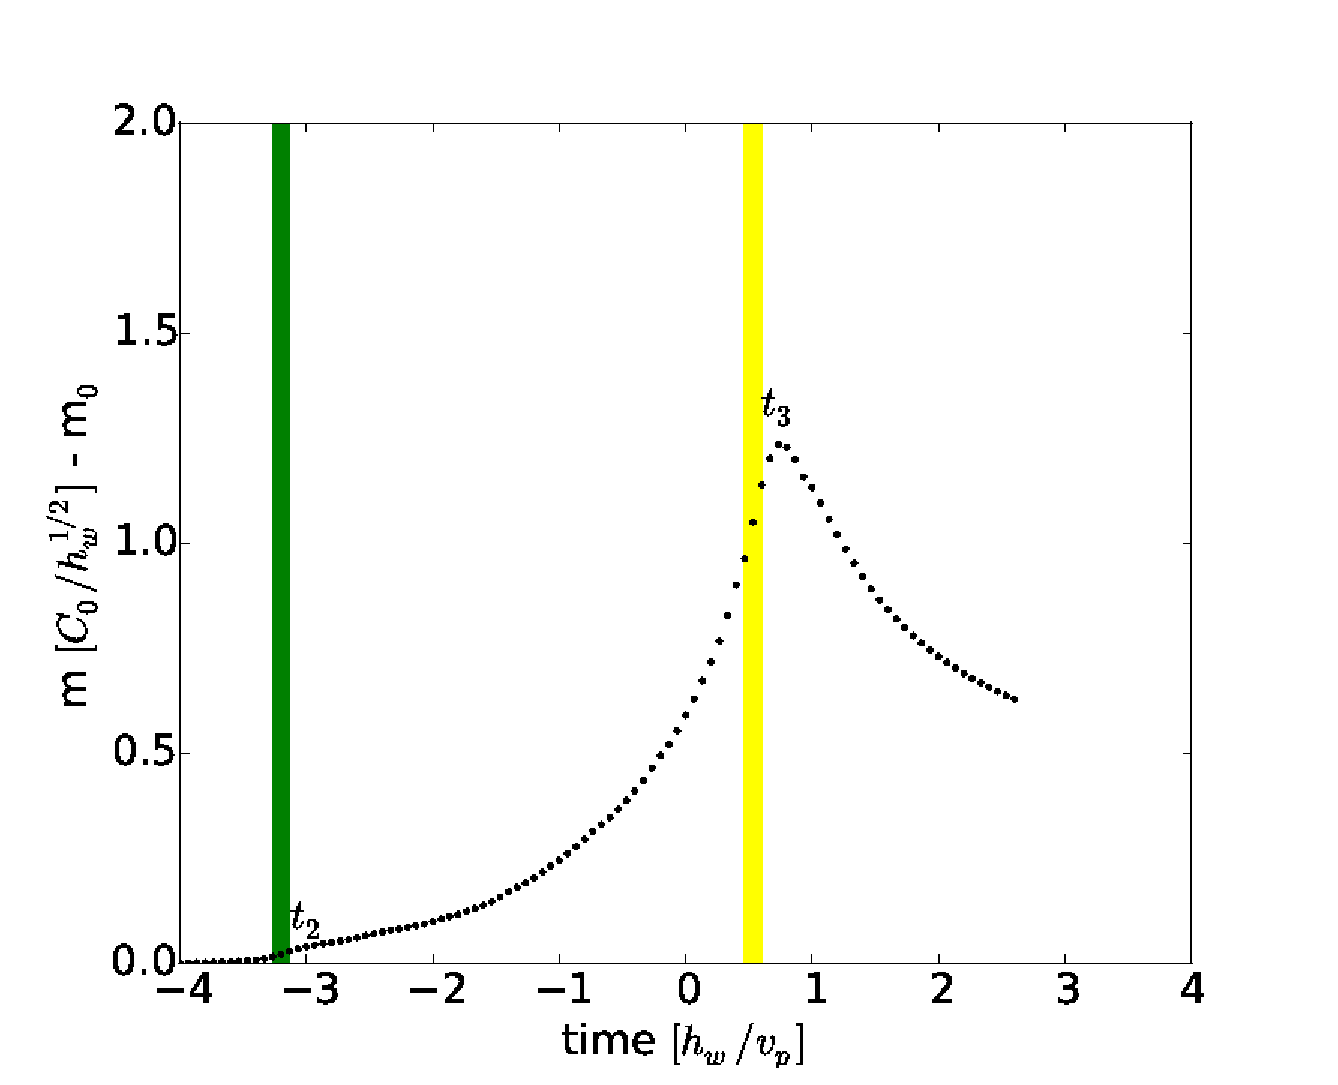
\includegraphics[width = 0.48\textwidth]{figures/M87_lc.eps}
\caption{\label{fig:M87_plots} The one dimensional profile obtained
  from the numerical integration along the ordonata axis of the source
  image (figure 9) is presented in the lower panel. The corresponding
  lightcurve associated to the 1D profile is presented in the right
  panel. The points p2 and p3 mark the start and end of the equivalent
  dark disk and are associated to the moments of their overlap with
  the caustic: t2 and t3.}
\end{figure}
